%====================================================================================
\section{Fronteras de utilidad}
%====================================================================================

\begin{frame}{La Frontera de Posibilidades de Utilidad $(FPU)$}
	\begin{figure}[h]
		\centering
		 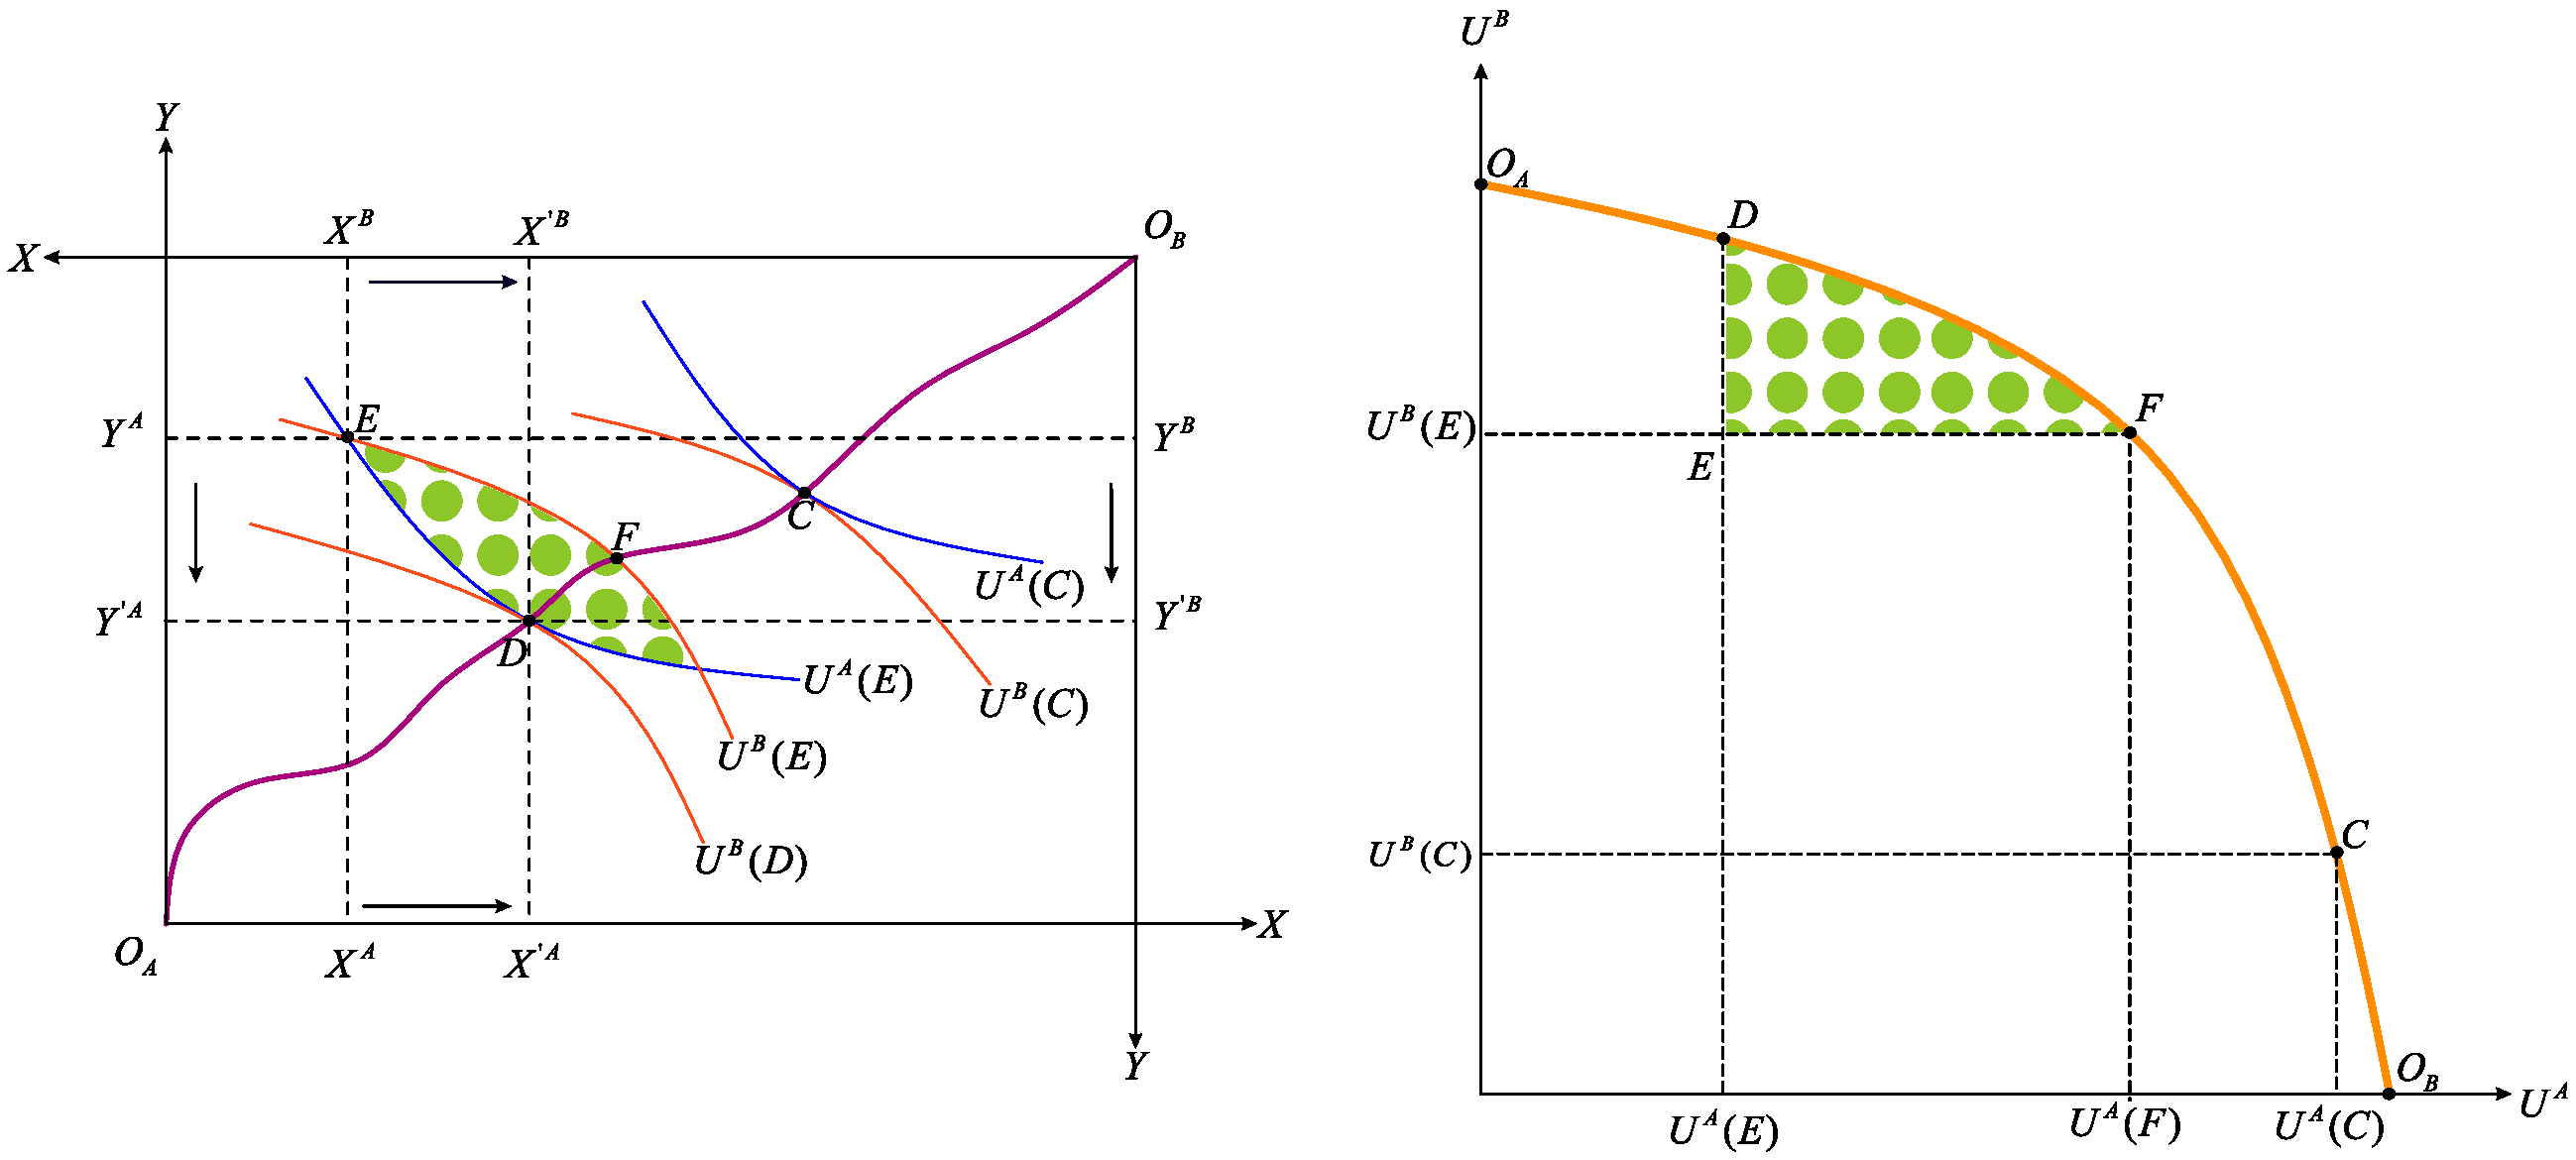
\includegraphics[width = 1\linewidth]{figures/fig_01.pdf}
	\end{figure}
\end{frame}
%------------------------------------------------
\begin{frame}{La Frontera de Posibilidades de Utilidad $(FPU)$}
	\begin{itemize}
		\item La Frontera de Posibilidades de Utilidad es la frontera más alta del conjunto de posibilidades de utilidad de la economía.
		\item Corresponde a los niveles de utilidad posibles en una caja de Edgeworth dada.
		\item Pero: la $FPU$ no es útil para economías con producción.
	\end{itemize}
\end{frame}
%------------------------------------------------
\begin{frame}{La Frontera de Posibilidades de Utilidad $(FPU)$}
D y F son asignaciones Pareto óptimas en una economía con producción, pero surgen de distintas cajas de Edgeworth , definidas por distintas combinaciones de productos.
	\begin{figure}[h]
		\centering
		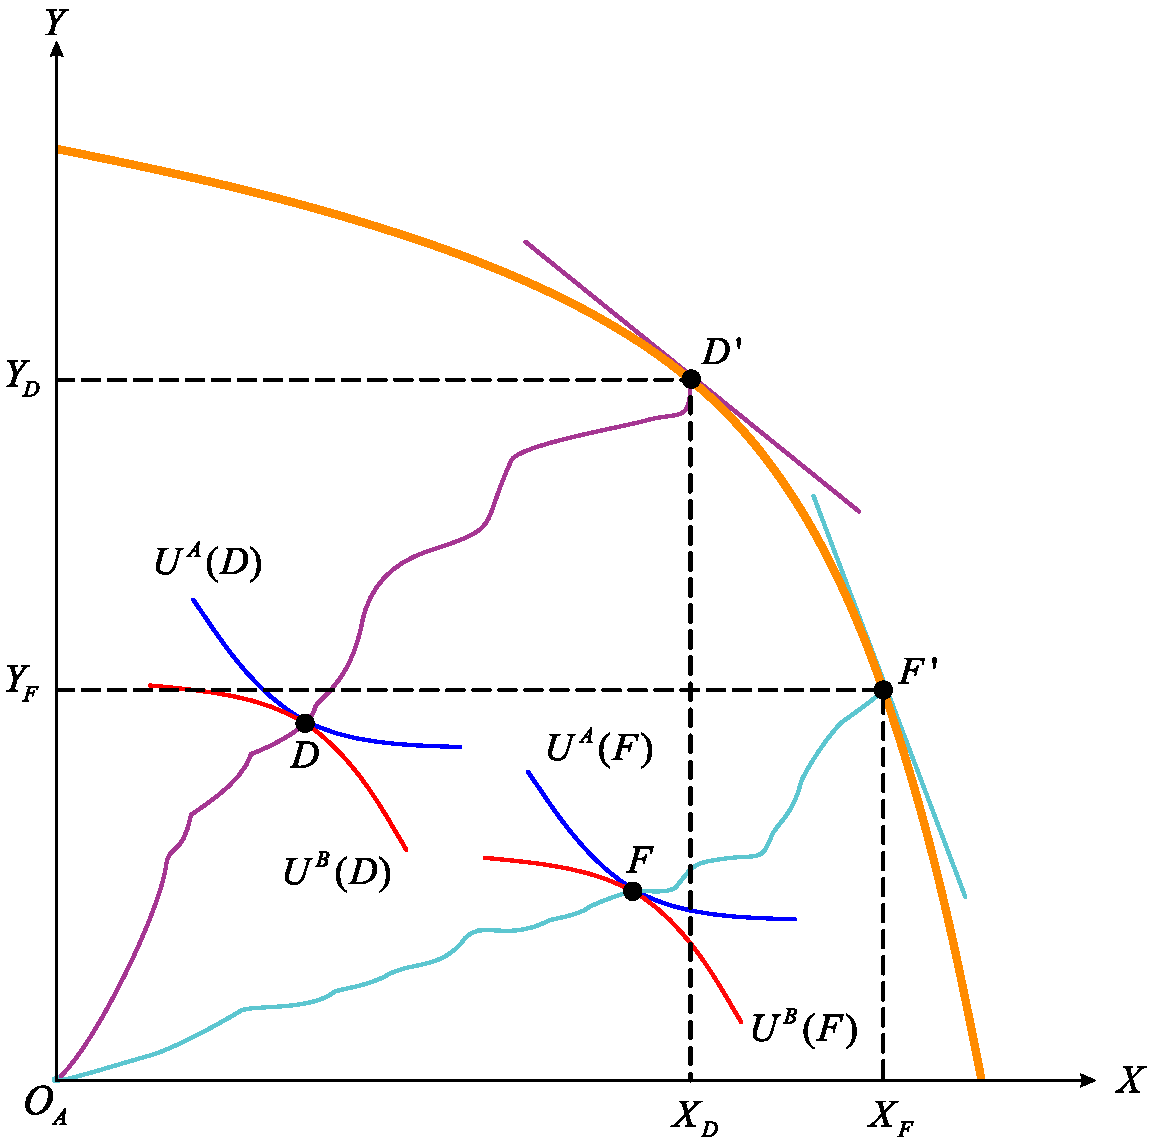
\includegraphics[width = 0.4\linewidth]{figures/fig_02.pdf}
	\end{figure}
Una $FPU$ se obtiene sólo para una única caja de Edgeworth, y la mayor parte de las asignaciones en una caja particular no son Pareto óptimos cuando la producción es considerada.
\end{frame}
%------------------------------------------------
\begin{frame}{La Frontera de Posibilidades de Utilidad $(FPU)$}
A fin de obtener una $FPU$ para una economía de producción necesitamos construir una ``Gran Frontera de Posibilidades de Utilidad'' $(GFPU)$
	\begin{figure}[h]
		\centering
		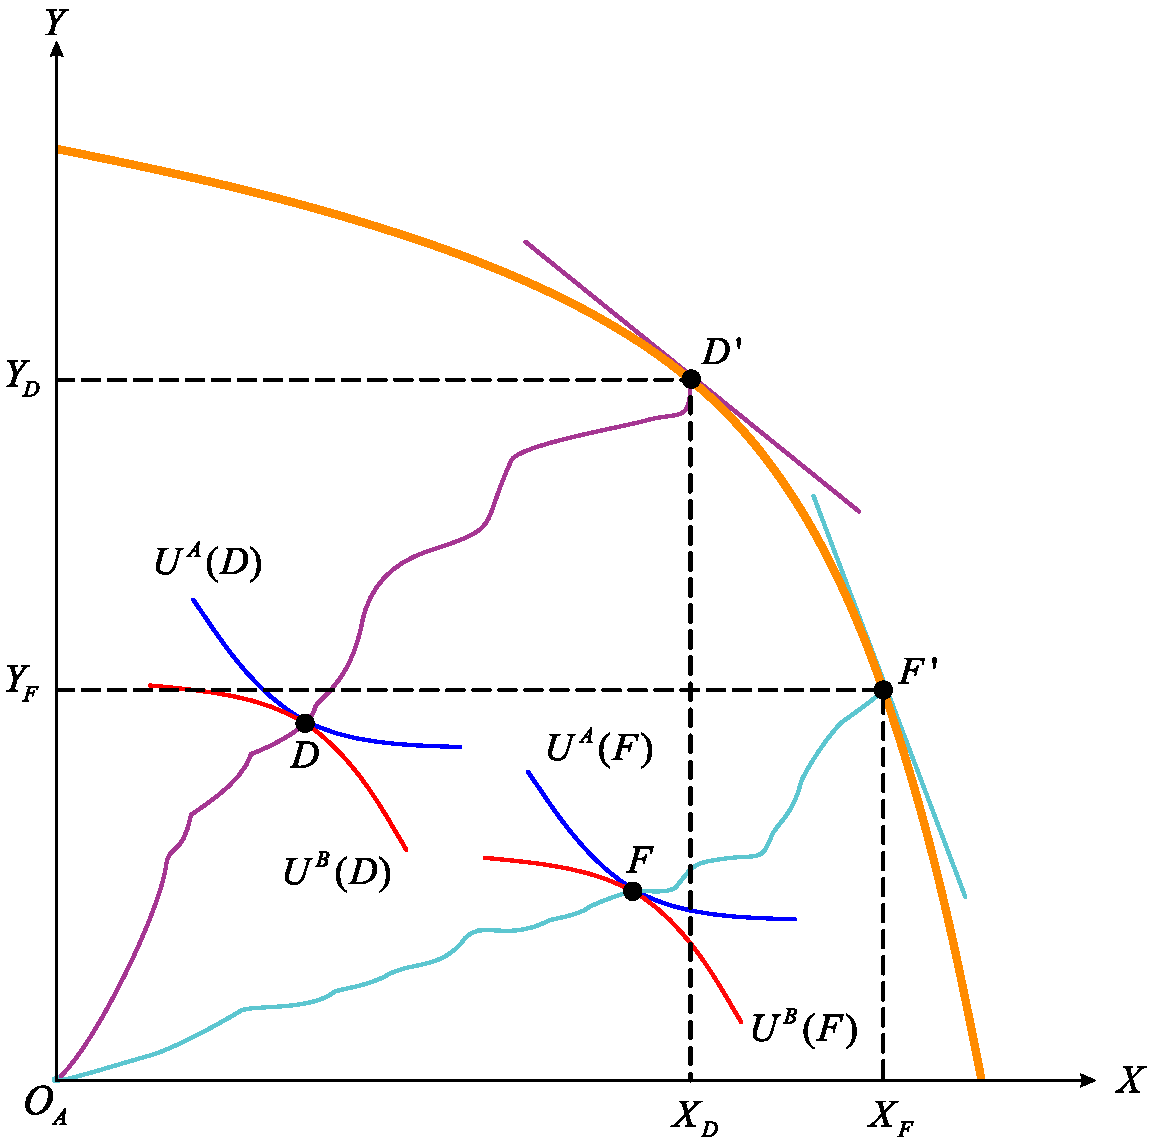
\includegraphics[width = 0.6\linewidth]{figures/fig_02.pdf}
	\end{figure}
\end{frame}
%------------------------------------------------
\begin{frame}{La Gran Frontera de Posibilidades de Utilidad $(GFPU)$}
La curva $FPU_F$ corresponde a la curva de contrato obtenida a partir de una caja de Edgeworth definida por la asignación $F'$.
	\begin{figure}[h]
		\centering
		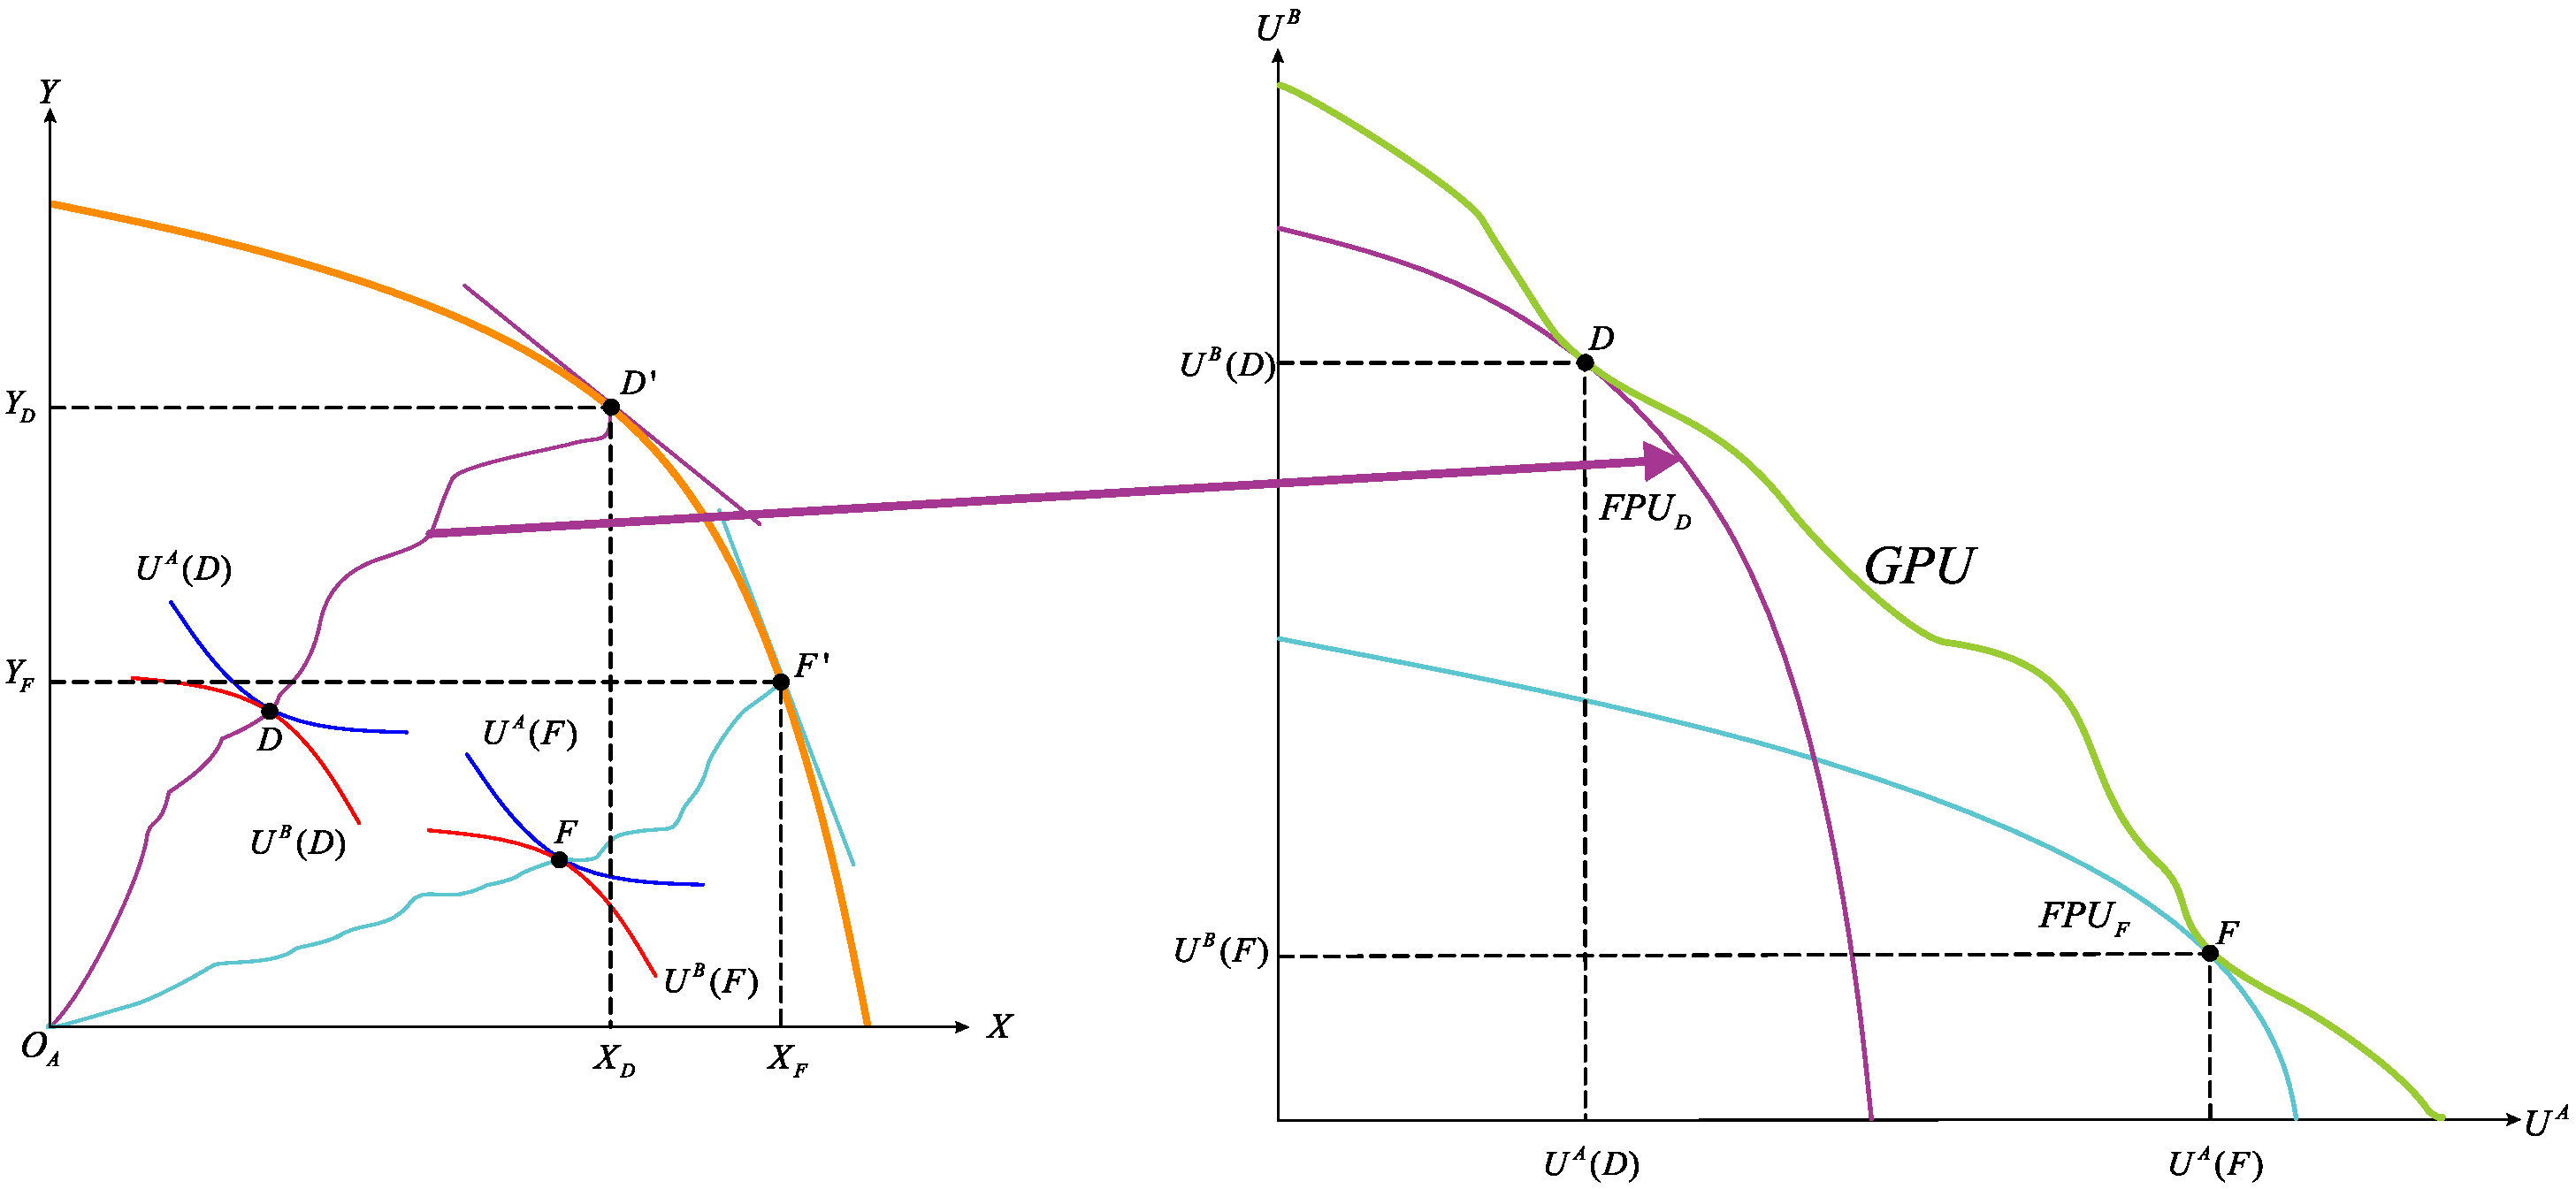
\includegraphics[width = 1\linewidth]{figures/fig_03.pdf}
	\end{figure}
\end{frame}
%------------------------------------------------
\begin{frame}{La Gran Frontera de Posibilidades de Utilidad $(GFPU)$}
La curva $FPU_D$ corresponde a la curva de contrato en la caja definida por la asignación $D'$.
	\begin{figure}[h]
		\centering
		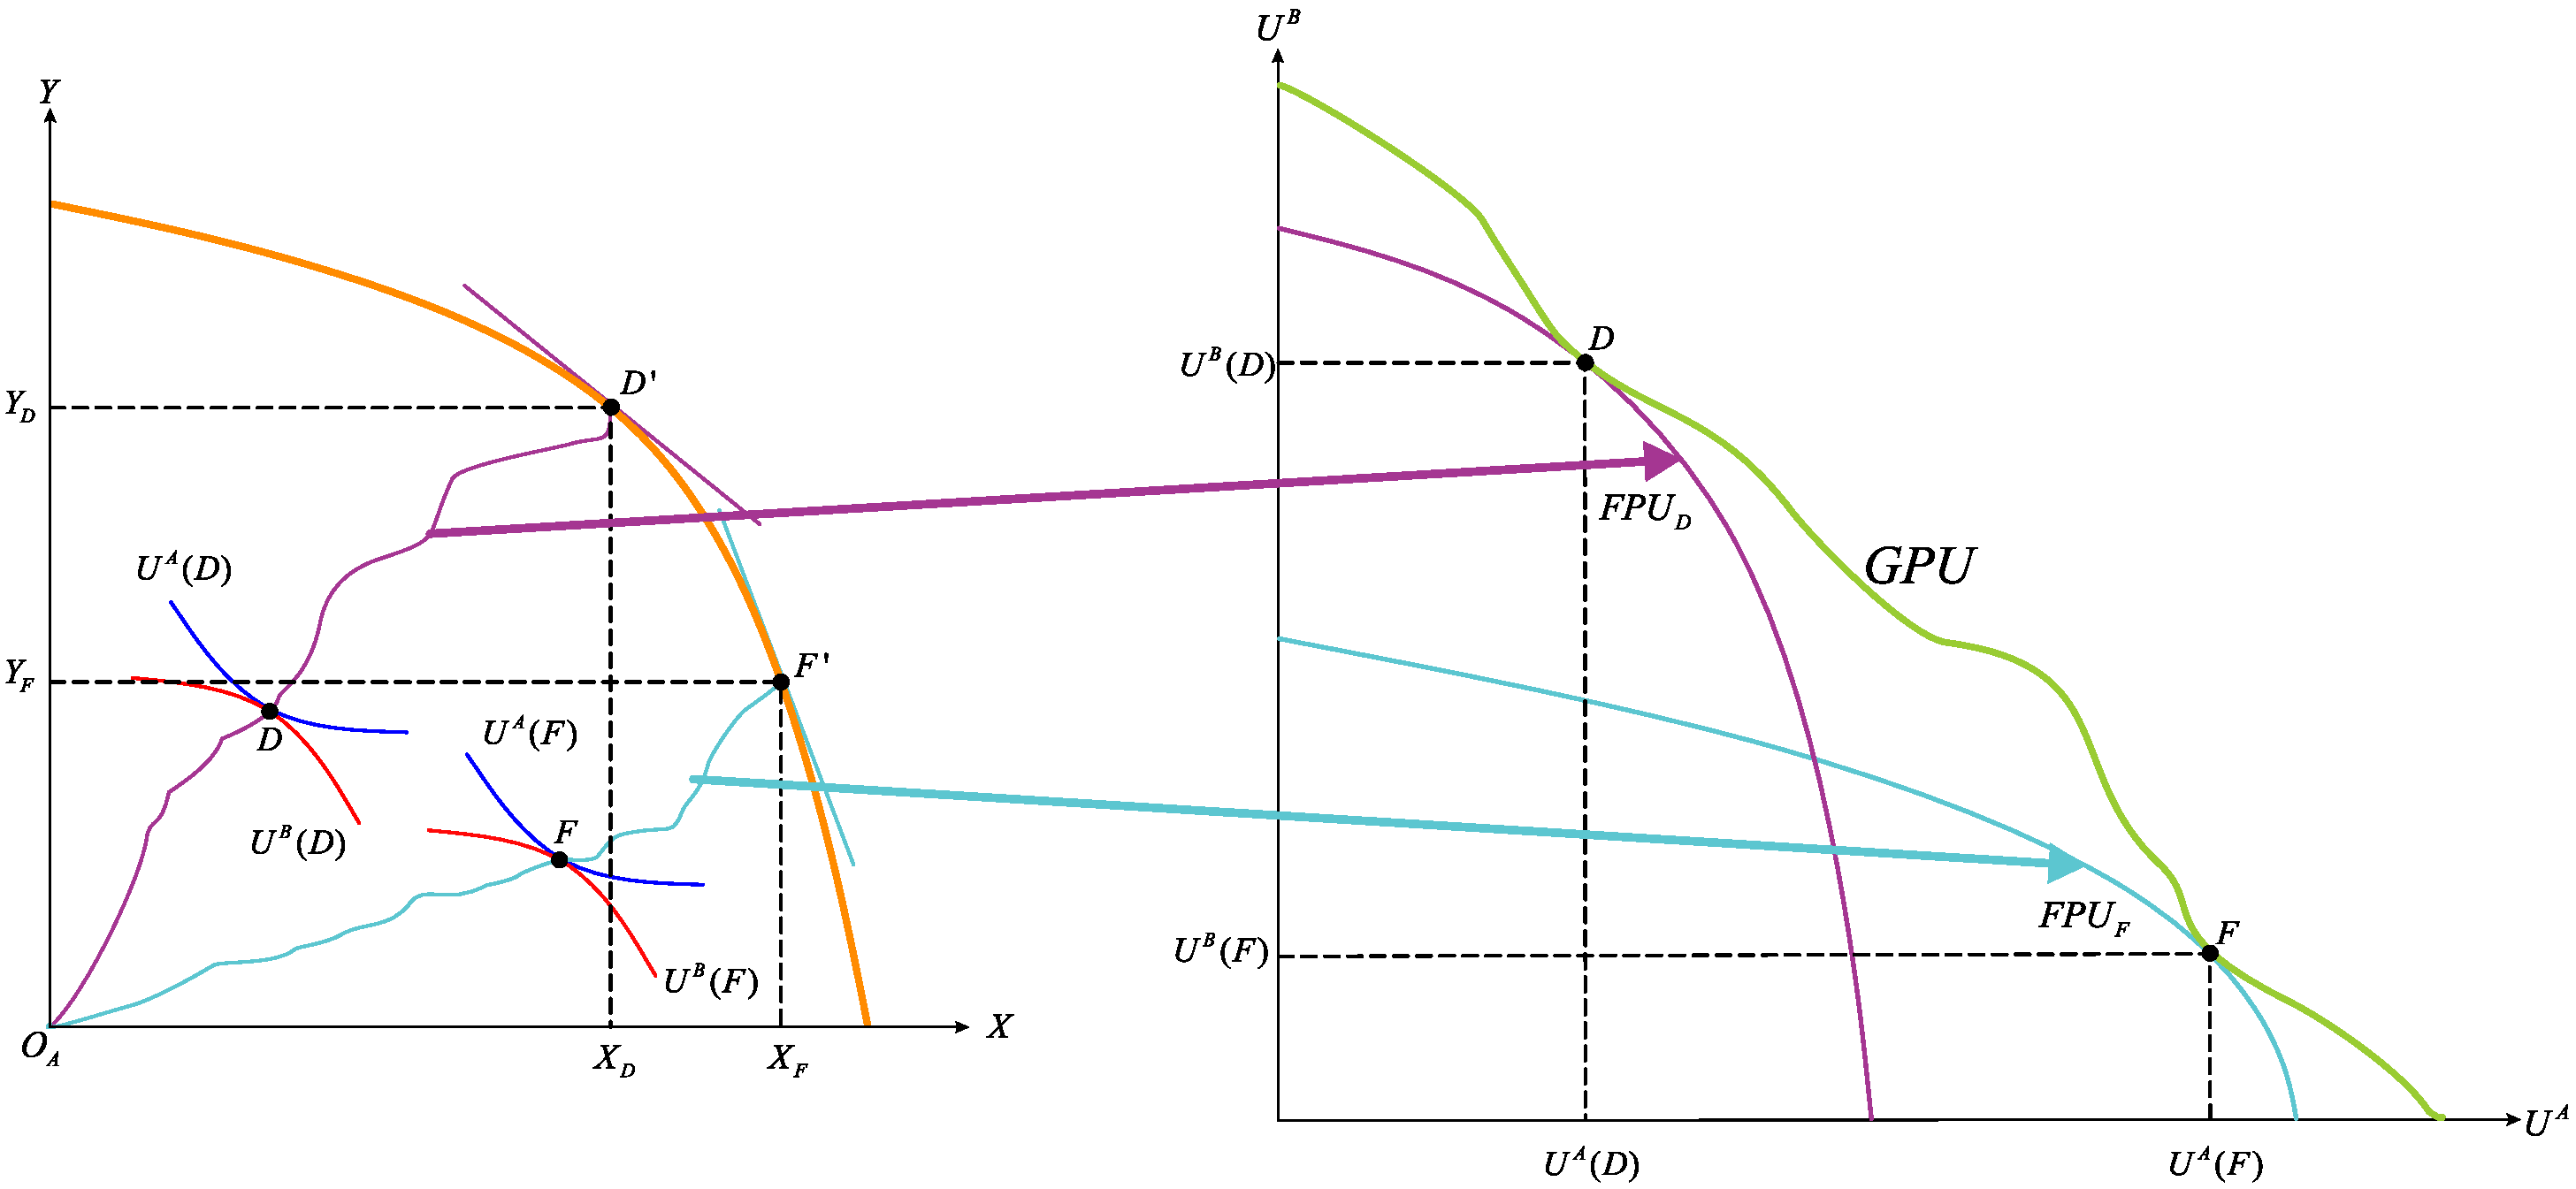
\includegraphics[width = 1\linewidth]{figures/fig_04.pdf}
	\end{figure}
\end{frame}
%------------------------------------------------
\begin{frame}{La Gran Frontera de Posibilidades de Utilidad $(GFPU)$}
El punto $F$ en $FPU_F$ y el punto $D$ en $FPU_D$ corresponden a las combinaciones de utilidad de los puntos $D$ y $F$.
	\begin{figure}[h]
		\centering
		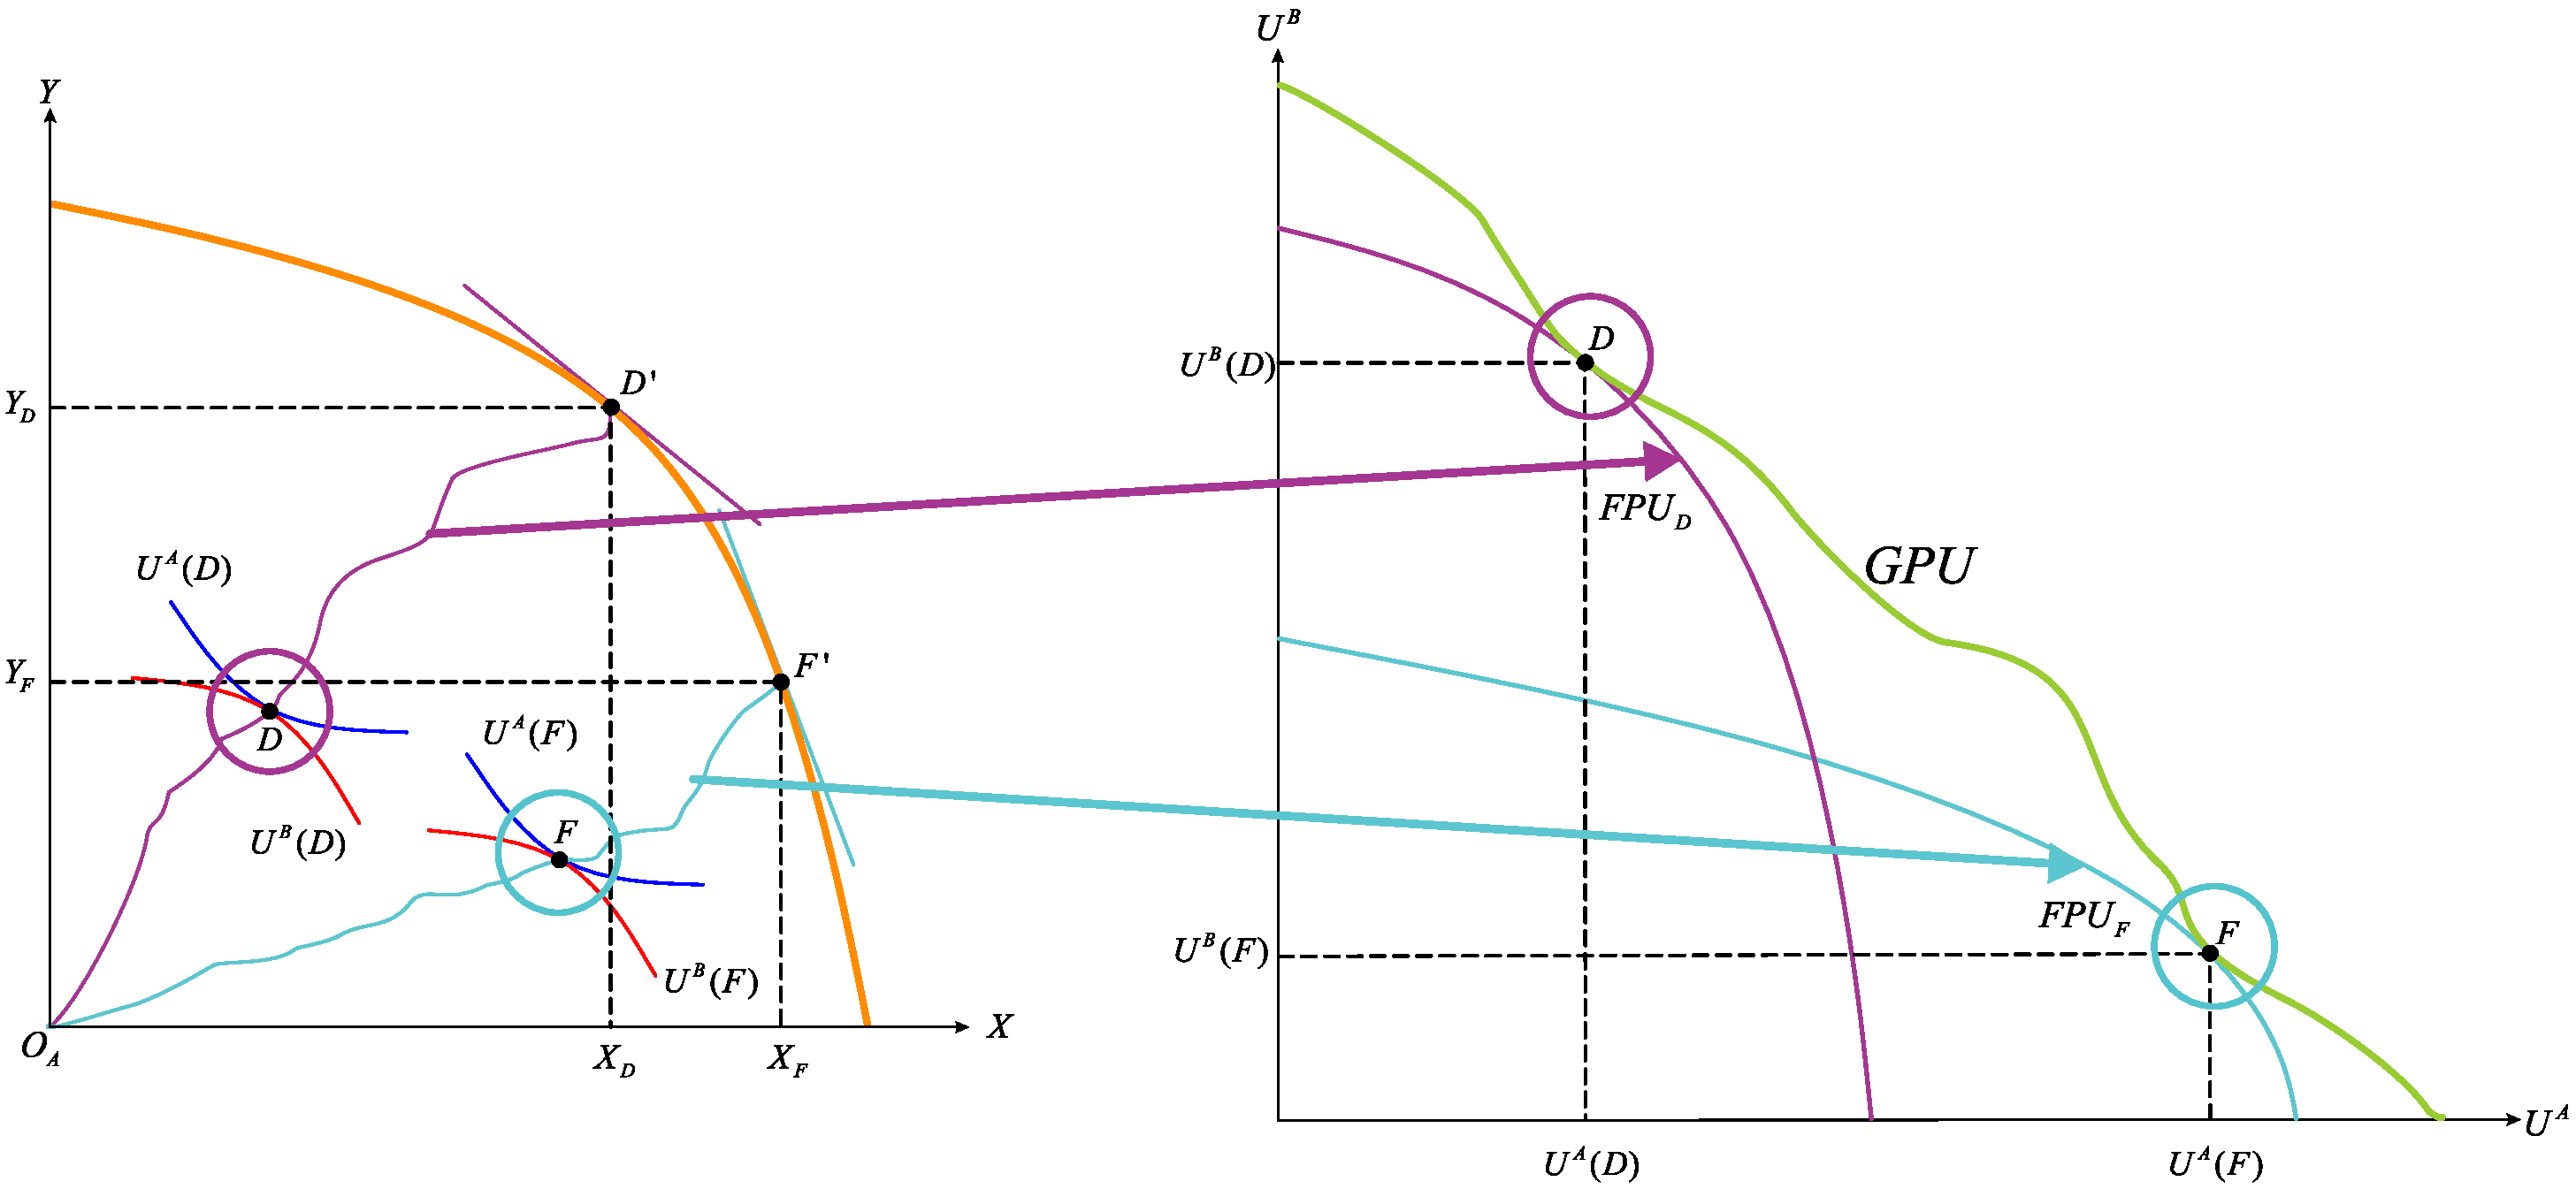
\includegraphics[width = 1\linewidth]{figures/fig_05.pdf}
	\end{figure}
\end{frame}
%------------------------------------------------
\begin{frame}{La Gran Frontera de Posibilidades de Utilidad $(GFPU)$}
Sólo $D$ y $F$ son asignaciones Pareto óptimas en sentido pleno (satisfacen $TMS=TMT$).
	\begin{figure}[h]
		\centering
		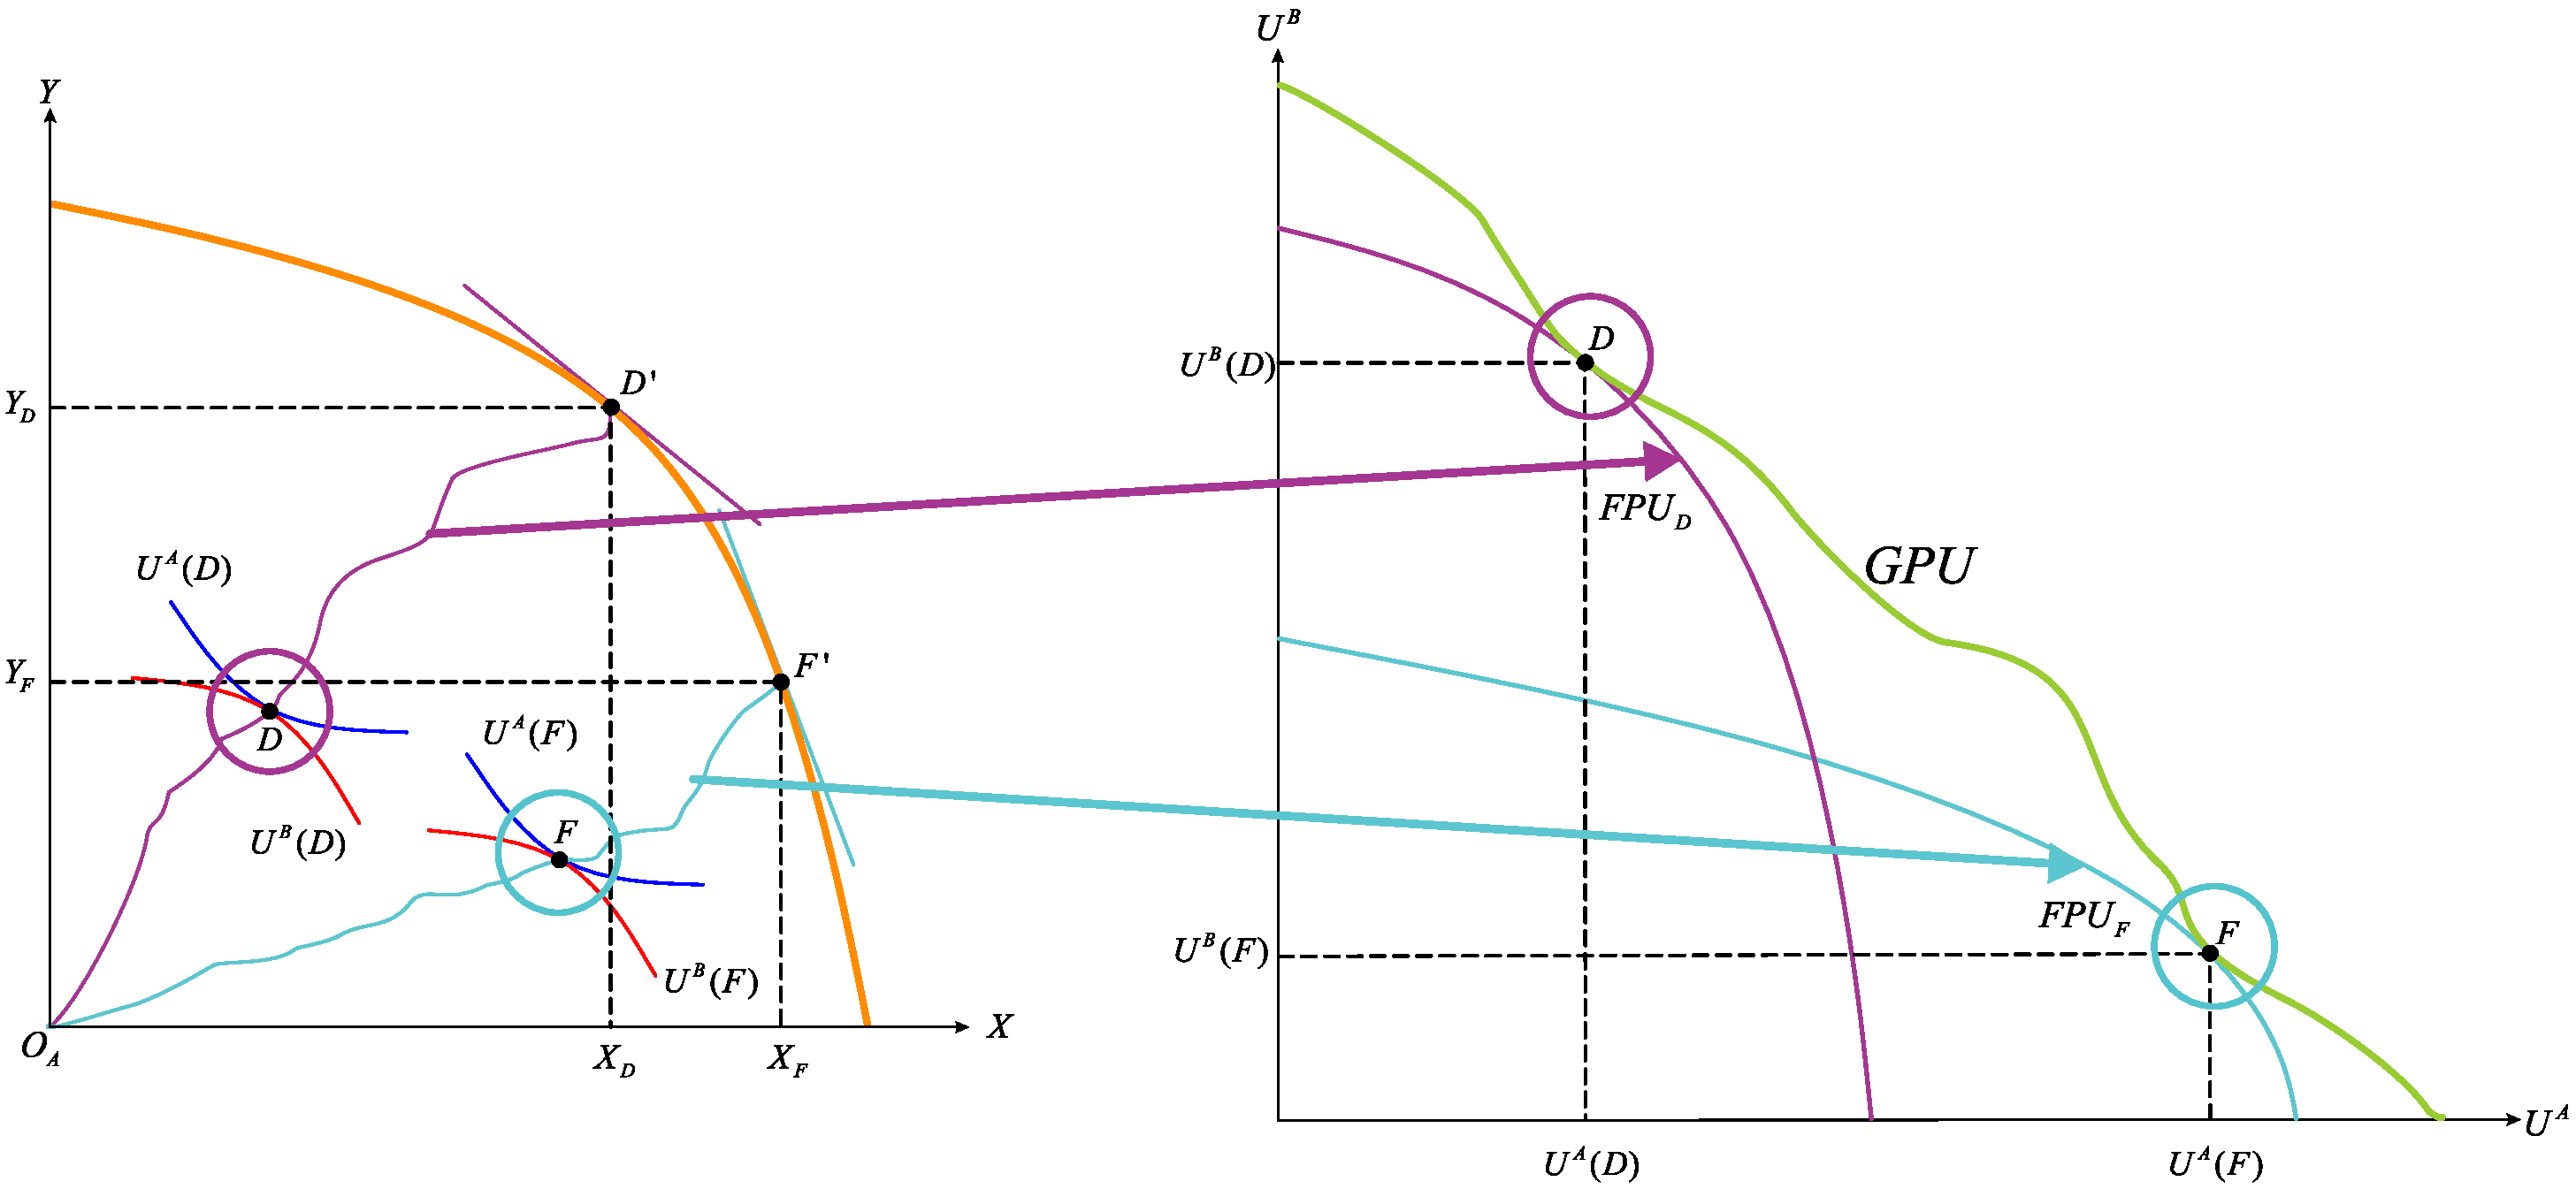
\includegraphics[width = 1\linewidth]{figures/fig_05.pdf}
	\end{figure}
\end{frame}
%------------------------------------------------
\begin{frame}{La Gran Frontera de Posibilidades de Utilidad $(GFPU)$}
Como cada asignación de producto da lugar a diferentes $FPU$, podemos reunir una serie de asignaciones y elaborar la $GFPU$ como la envolvente de las $FPU$ que pasa a través de asignaciones Pareto óptimas plenas como $D$ y $F$.
	\begin{figure}[h]
		\centering
		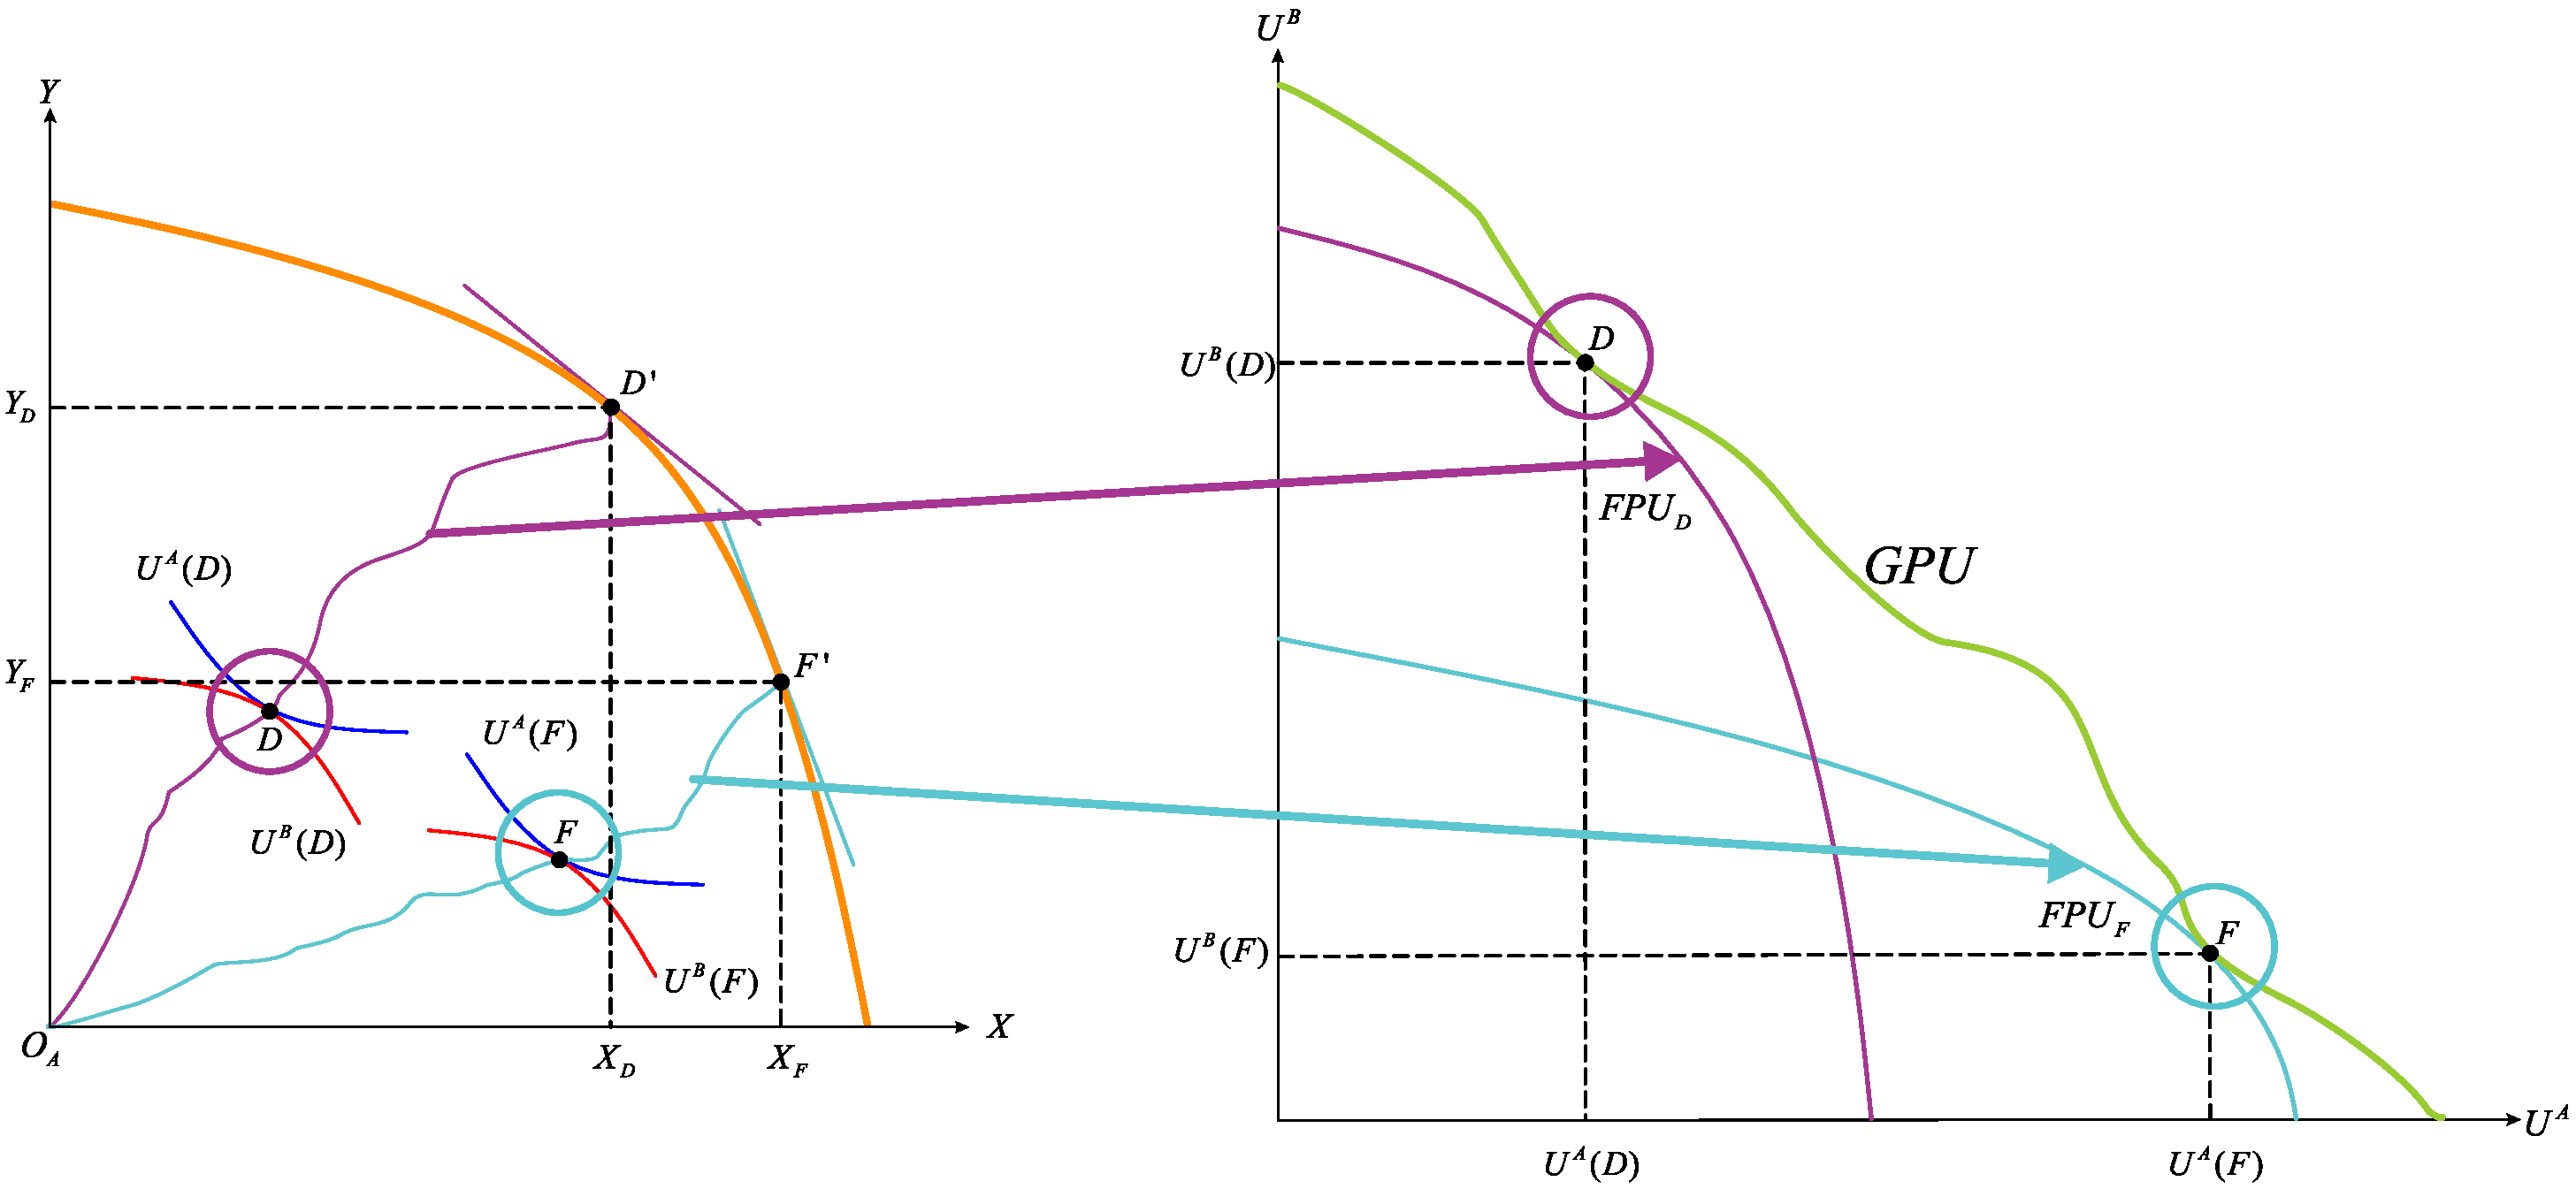
\includegraphics[width = 1\linewidth]{figures/fig_05.pdf}
	\end{figure}
\end{frame}
%------------------------------------------------
\begin{frame}{La Gran Frontera de Posibilidades de Utilidad $(GFPU)$}
	Para estar sobre la Gran Frontera de Posibilidades de Utilidad, la Tasa Marginal de Transformación en un punto de la Frontera de Posibilidades de Producción, debe igualar a la relación marginal de sustitución (igualada) de las curvas (o contornos) de indiferencia) a lo largo del conjunto paretiano asociado con el punto de la $FPP$.
\end{frame}
%------------------------------------------------
\begin{frame}{La Gran Frontera de Posibilidades de Utilidad $(GFPU)$}
	\begin{figure}[!h]
		\centering
		 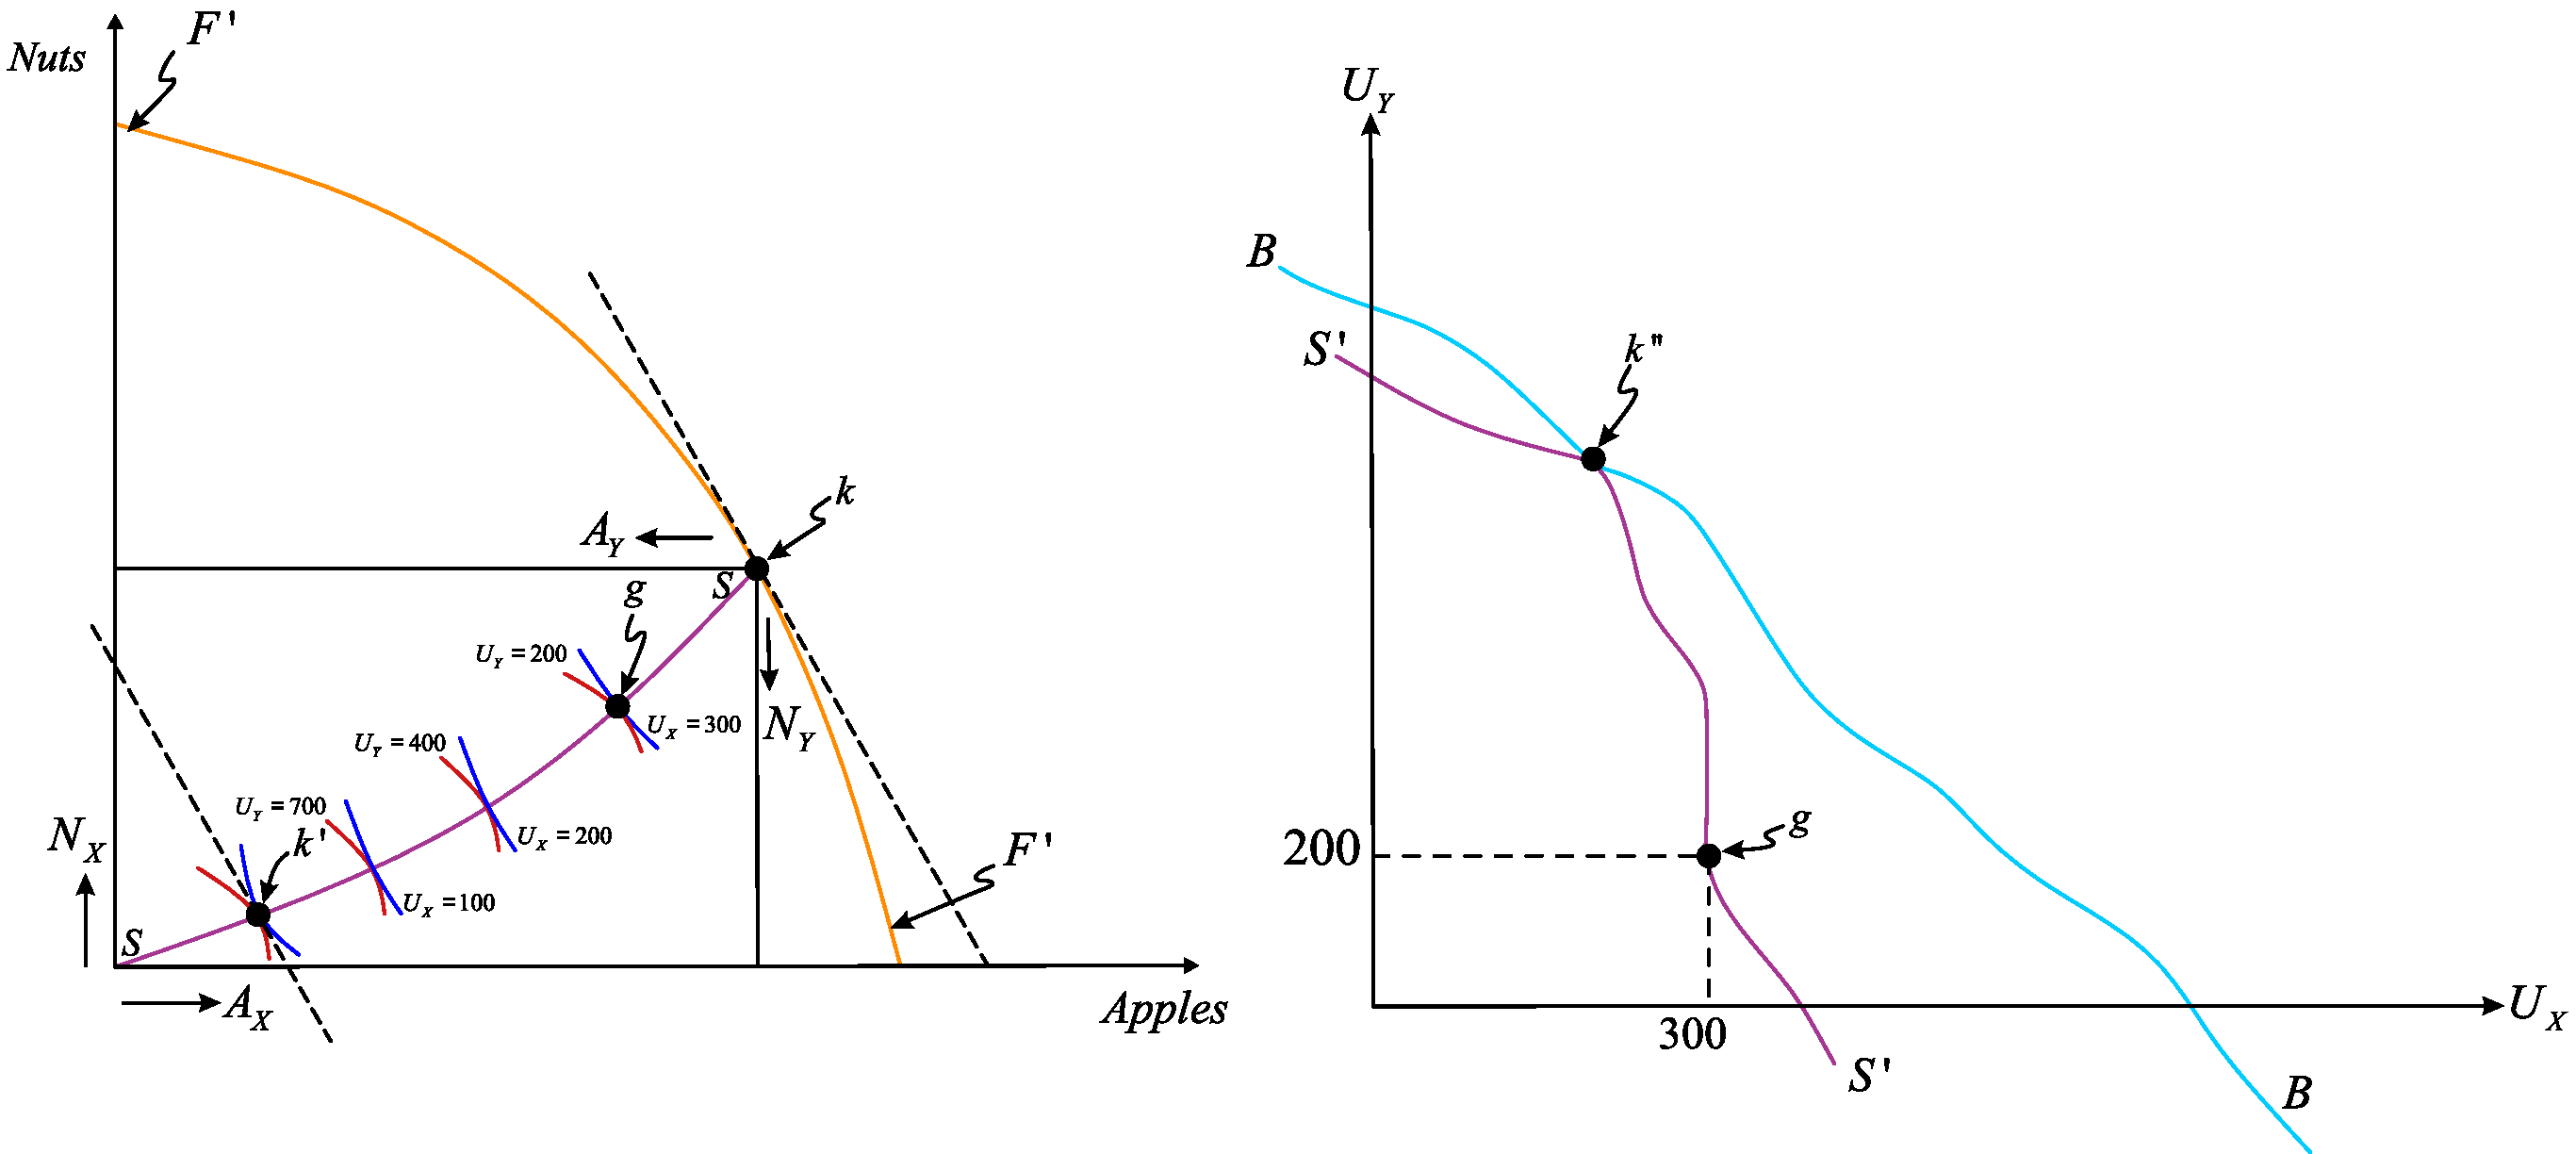
\includegraphics[width = 1\linewidth]{figures/fig_06.pdf}
	\end{figure}
\end{frame}
%------------------------------------------------
\begin{frame}{De la $GFPU$ a la maximización de la Función de Bienestar Social}
	\begin{figure}[!h]
		\centering
		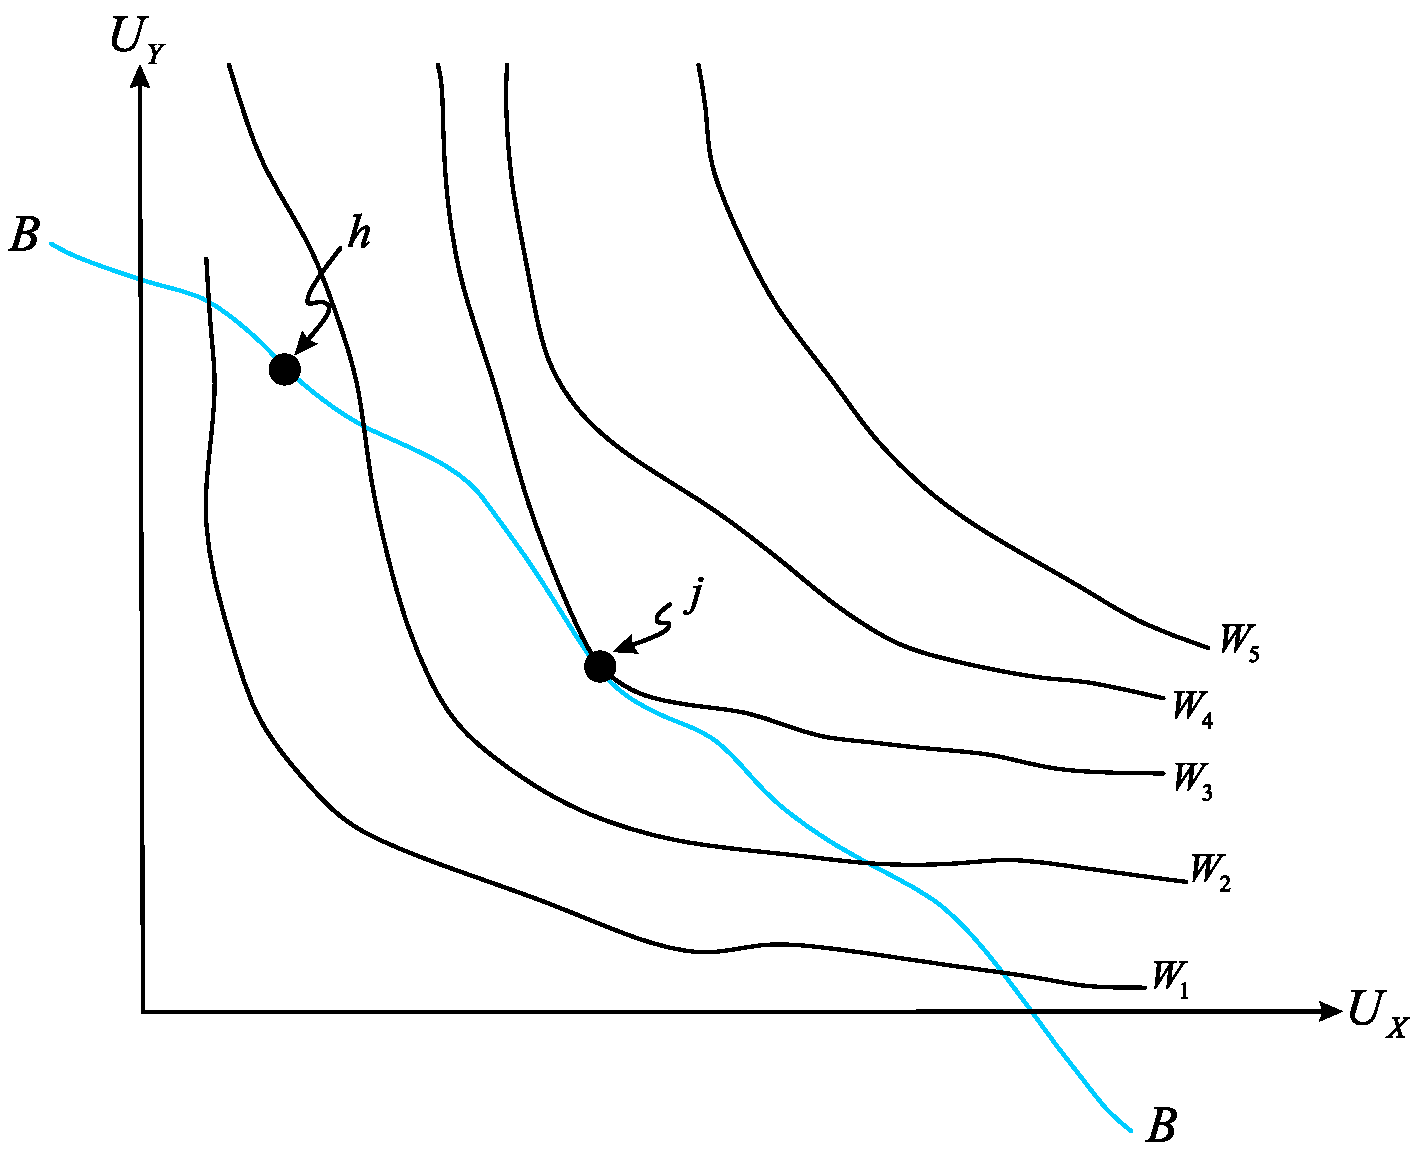
\includegraphics[width = 0.8\linewidth]{figures/fig_07.pdf}
	\end{figure}
\end{frame}